% 2026_beijing_q18_fig1: 直三棱柱 ABC-A1B1C1，D 为 AC 中点，E 为 A1B1 中点，P 在顶面内
\usetikzlibrary{calc}
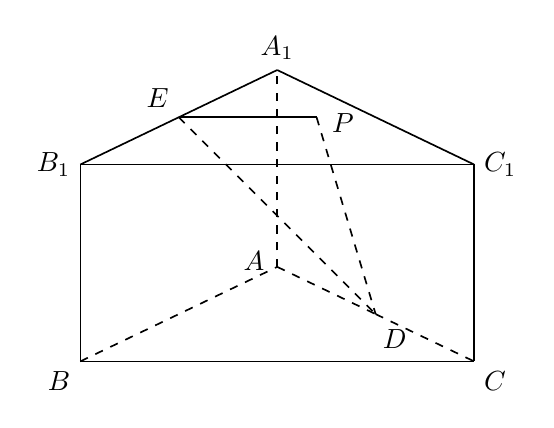
\begin{tikzpicture}[x=1cm,y=1cm,line width=.6pt]
  \coordinate (B) at (0,0);
  \coordinate (C) at (5,0);
  \coordinate (A) at (2.5,1.2);
  \coordinate (B1) at (0,2.5);
  \coordinate (C1) at (5,2.5);
  \coordinate (A1) at (2.5000000000,3.7000000000);
  \coordinate (E) at (1.2500000000,3.1000000000);
  \coordinate (D) at (3.75,0.6);
  \coordinate (P) at (3.0000000000,3.1000000000);
  % 底面：BC 可见，AB/AC 遮挡（D 在 AC 上）
  \draw (B) -- (C);
  \draw[dashed] (B) -- (A);
  \draw[dashed] (A) -- (D);
  \draw[dashed] (D) -- (C);
  % 侧棱：BB1/CC1 可见，AA1 遮挡
  \draw (B) -- (B1);
  \draw (C) -- (C1);
  \draw[dashed] (A) -- (A1);
  % 顶面
  \draw (B1) -- (C1);
  \draw (B1) -- (A1);
  \draw (C1) -- (A1);
  % 附加线段
  \draw[dashed] (E) -- (D);
  \draw (E) -- (P);
  \draw[dashed] (P) -- (D);
  % 标签
  \node[below left,font=\normalsize] at (B) {$B$};
  \node[below right,font=\normalsize] at (C) {$C$};
  \node[left,font=\normalsize,xshift=-1.0pt,yshift=2pt] at (A) {$A$};
  \node[left,font=\normalsize] at (B1) {$B_1$};
  \node[right,font=\normalsize] at (C1) {$C_1$};
  \node[above,font=\normalsize] at (A1) {$A_1$};
  \node[above left,font=\normalsize] at (E) {$E$};
  \node[below right,font=\normalsize,xshift=-1.0pt,yshift=-2pt] at (D) {$D$};
  \node[right=2pt,xshift=0.000pt,yshift=-2.008pt] at (P) {$P$};
\end{tikzpicture}
